% Standalone rendering of every figure in the paper, so the figure sources in
% this repository can be built and checked without the manuscript.
%
%   cd paper && pdflatex -interaction=nonstopmode figures.tex
%
% Data comes from ../data/pgfplots, which the pipeline writes. twocolumn is
% required because four of the six are figure* (full-width) environments.
% The tikz/pgfplots setup below matches the manuscript preamble, so the
% figures render as they do in the paper.
\documentclass[twocolumn,10pt]{article}
\usepackage[margin=2cm]{geometry}
\usepackage{graphicx}
\usepackage{textcomp}
\usepackage{amsmath}
\usepackage[dvipsnames]{xcolor}
\usepackage{tikz}
\usetikzlibrary{arrows.meta, positioning}
\usepackage{pgfplots}
\usepackage{pgfplotstable}
\pgfplotsset{compat=1.18,
  every axis/.append style={
    /pgf/number format/1000 sep={},
    /pgf/number format/fixed,
  }
}
\usepgfplotslibrary{groupplots}
\usepackage{caption}

\title{abstract-audit: figure sources}
\author{}
\date{}

\begin{document}
\maketitle

% Overview of the setup. One corpus, two scoring paths, opposite
% verdicts. Compact two-column float. Self-contained: defines its own
% colors and styles. Requires tikzlibrary arrows.meta, positioning and
% pgfplots (both loaded by the manuscript).
\definecolor{Navy}{HTML}{173B67}
\definecolor{Blue}{HTML}{2F6FA8}
\definecolor{BlueLight}{HTML}{E8F1F9}
\definecolor{Orange}{HTML}{B45608}
\definecolor{OrangeDark}{HTML}{A95B06}
\definecolor{OrangeLight}{HTML}{FCEFE0}
\definecolor{Teal}{HTML}{12615F}
\definecolor{Ink}{HTML}{172033}
\definecolor{Rule}{HTML}{93A2B0}
\definecolor{Panel}{HTML}{F4F7FA}

\tikzset{
  ovcard/.style={rounded corners=1.5mm, draw=Rule, fill=Panel,
                 line width=.5pt, inner sep=1.5mm, align=center,
                 font=\fontsize{8}{9.4}\selectfont, text=Ink},
  ovflow/.style={-{Latex[length=1.6mm,width=1.7mm]}, line width=.6pt},
  ovnote/.style={font=\fontsize{6.6}{7.6}\selectfont, text=Ink!85,
                 align=left, anchor=west},
}
% Emphasis for the card headings. Must be a macro, not a tikz style: it is
% used inside node text as {\ovtag ...}, which a pgfkeys style cannot serve.
\providecommand{\ovtag}{}
\renewcommand{\ovtag}{\bfseries\fontsize{8}{9.4}\selectfont}

\pgfplotsset{
  ovaxis/.style={
    width=3.10cm, height=1.34cm, scale only axis,
    axis line style={draw=Ink!70,line width=.4pt},
    tick style={draw=Ink!70,line width=.35pt},
    tick align=outside, tick pos=left,
    xtick={1987,2005,2025},
    xticklabel style={/pgf/number format/1000 sep={}},
    tick label style={font=\fontsize{5.8}{6.4}\selectfont,text=Ink!85},
    xmin=1984, xmax=2028,
    clip=false, grid=none, axis on top,
  }
}

\begin{figure*}[t]
\centering
{\sffamily
\begin{tikzpicture}[x=1cm,y=1cm]

% ---- Corpus card (left) -------------------------------------------
\node[ovcard, text width=2.05cm, align=center, minimum height=1.9cm] (corpus) at (0,0)
  {{\ovtag NeurIPS abstracts}\\[.5mm] 30,595 papers\\ 1987--2025\\[.6mm]
   {\fontsize{7}{8}\selectfont abstracts only}};

% ---- Path cards ----------------------------------------------------
\node[ovcard, draw=Blue, fill=BlueLight, minimum width=3.0cm,
      minimum height=1.05cm, anchor=west] (ref) at (1.55,1.30)
  {{\ovtag\color{Navy} Human-grounded}\\
   {\ovtag\color{Navy} reference}\\[.3mm]
   15 classical formulas};
\node[ovcard, draw=Orange, fill=OrangeLight, minimum width=3.0cm,
      minimum height=1.05cm, anchor=west] (judge) at (1.55,-1.30)
  {{\ovtag\textcolor{Orange}{LLM-as-a-judge}}\\[.3mm]
   6 models $\times$ 3 prompts};

\draw[ovflow, Blue]   (corpus.east) -- (1.30,0) |- (ref.west);
\draw[ovflow, Orange] (corpus.east) -- (1.30,0) |- (judge.west);
\draw[ovflow, Blue]   (ref.east)   -- ++(.30,0);
\draw[ovflow, Orange] (judge.east) -- ++(.30,0);

% ---- Trend charts (shared x axis, labelled once below) -------------
\node[font=\fontsize{7}{8}\selectfont, text=Navy, anchor=south west]
  at (5.25,1.88) {Flesch Reading Ease ($\uparrow$ easier)};
\begin{axis}[ovaxis, at={(5.25cm,0.44cm)}, anchor=south west,
  ymin=5, ymax=31, ytick={10,20,30}, xticklabels={}]
  \addplot[Blue, line width=.9pt, mark=*, mark size=.85pt,
           mark options={fill=Blue,draw=Blue}]
    table[x=year,y=flesch,col sep=comma]{../data/pgfplots/va_flesch.csv};
  \draw[Ink!45,densely dotted,line width=.45pt]
    (axis cs:2022,5)--(axis cs:2022,31);
\end{axis}

\node[font=\fontsize{7}{8}\selectfont, text=Orange, anchor=south west]
  at (5.25,-0.60) {Judge score ($z$, model averaged)};
\begin{axis}[ovaxis, at={(5.25cm,-1.94cm)}, anchor=south west,
  ymin=-1.3, ymax=4.0, ytick={0,2,4}]
  \addplot[OrangeDark, line width=.9pt, mark=*, mark size=.85pt,
           mark options={fill=OrangeDark,draw=OrangeDark}]
    table[x=year,y=z,col sep=comma]{../data/pgfplots/va_zscore.csv};
  \draw[Ink!45,densely dotted,line width=.45pt]
    (axis cs:2022,-1.3)--(axis cs:2022,4.0);
\end{axis}
\node[font=\fontsize{6.2}{7}\selectfont, text=Ink!70, anchor=north]
  at (6.80,-2.46) {dotted line marks late 2022};

% ---- Per-path verdicts ---------------------------------------------
\node[ovnote, text=Navy, font=\bfseries\fontsize{7.4}{8.4}\selectfont]
  at (8.60,1.32) {declines};
\node[ovnote] at (8.60,0.84) {harder to read,\\ all 15 agree};

\node[ovnote, text=Orange, font=\bfseries\fontsize{7.4}{8.4}\selectfont]
  at (8.60,-1.10) {flat, then rises};
\node[ovnote] at (8.60,-1.60) {judged easier,\\ all $6\times3$ agree};

% ---- Verdict (right) -----------------------------------------------
\draw[Rule, line width=.5pt] (10.85,1.60) -- (11.10,1.60)
  -- (11.10,-1.60) -- (10.85,-1.60);
\draw[Rule, line width=.5pt] (11.10,0) -- (11.35,0);

\node[ovcard, draw=Teal, fill=white, line width=.7pt, anchor=west,
      minimum height=2.3cm, text width=3.0cm, align=left]
  (verdict) at (11.35,0)
  {\hyphenpenalty=10000\exhyphenpenalty=10000
   {\ovtag\textcolor{Teal}{Same corpus,\\ opposite direction.}}\\[1mm]
   The judges agree with each other but not with the reference. So
   agreement is not evidence of validity.};

\end{tikzpicture}%
}
\caption{\textbf{Overview of the setup.} One corpus of 30,595 NeurIPS
  abstracts (1987--2025) is scored along two independent paths, 15 classical
  readability formulas calibrated on human reading performance, and six open-weight
  instruction-tuned models under three prompt templates, standardized
  per model. The reference falls (reading gets harder) while the judges are
  flat and then rise after 2022 (text is judged easier).}
\label{fig:visual-abstract}
\end{figure*}

% Flesch Reading Ease on NeurIPS abstracts (body figure, NeurIPS only).
% Cross-venue and all-15-metric versions are in the appendix.
% Data: ../data/pgfplots/readability_flesch_ease.csv
% Higher values = easier reading.

\begin{figure}[t]
\centering
\begin{tikzpicture}
\begin{axis}[
    width=0.92\linewidth, height=5cm,
    xlabel={Year},
    ylabel={Flesch Reading Ease (\textuparrow\ easier)},
    xtick distance=4,
    x tick label style={rotate=45, anchor=east, font=\tiny,
                        /pgf/number format/1000 sep={}},
    ytick align=inside,
    tick label style={font=\tiny},
    label style={font=\small},
    enlarge x limits=0.02,
  ]
  \addplot[color={rgb,255:red,44;green,160;blue,44}, solid, very thick]
    table[x=year, y=neurips, col sep=comma]
    {../data/pgfplots/readability_flesch_ease.csv};
  % ChatGPT launch marker (late 2022)
  \draw[black, dashed, semithick] (axis cs:2022,-5) -- (axis cs:2022,50);
  \node[font=\tiny, rotate=90, anchor=south west]
    at (axis cs:2022.2,18) {ChatGPT (2022)};
\end{axis}
\end{tikzpicture}
\caption{\textbf{Flesch Reading Ease on NeurIPS abstracts,
  1987--2025.}
  Higher values indicate easier reading (\textuparrow). NeurIPS
  falls from approximately 24 in 1987 to approximately 8 in 2025,
  a sustained decline. All 15 classical metrics move in the same
  direction on NeurIPS (Appendix~\ref{app:readability}). Vertical dashed line marks the
  late-2022 availability of widely-used instruction-tuned writing
  assistants.}
\label{fig:readability-flesch}
\end{figure}

% Classical readability on NeurIPS only, appendix, split into two 3-column
% figures. Data: ../data/pgfplots/readability_<metric>.csv (neurips column).

\providecommand{\readpanel}[3]{%
  \nextgroupplot[title={\tiny #1~[#3]},
                 title style={font=\tiny, yshift=-1.5mm}]
  \addplot[color={rgb,255:red,44;green,160;blue,44}, dashdotted, very thick]
    table[x=year, y=neurips, col sep=comma]{../data/pgfplots/#2.csv};
  \draw[black, dashed, semithick]
    ({axis cs:2022,0} |- {rel axis cs:0,0})
    -- ({axis cs:2022,0} |- {rel axis cs:0,1});
}

% ── Figure A: 8 readability metrics, 3 by 3 layout (1 blank slot) ────────────
\begin{figure*}[t]
\centering
\begin{tikzpicture}
\begin{groupplot}[
    group style={
      group size=3 by 3,
      horizontal sep=8mm,
      vertical sep=12mm,
    },
    width=40mm, height=2.4cm,
    scale only axis,
    xlabel={}, ylabel={},
    xtick distance=12,
    x tick label style={rotate=55, anchor=east, font=\tiny,
                        /pgf/number format/1000 sep={}},
    y tick label style={font=\tiny},
    ytick align=inside,
    enlarge x limits=0.02,
    tick label style={font=\tiny},
  ]
  \readpanel{Flesch Ease}{readability_flesch_ease}{\textuparrow}
  \readpanel{Flesch--Kincaid}{readability_flesch_kincaid}{\textdownarrow}
  \readpanel{Gunning Fog}{readability_gunning_fog}{\textdownarrow}
  \readpanel{SMOG}{readability_smog}{\textdownarrow}
  \readpanel{Dale--Chall}{readability_dale_chall}{\textdownarrow}
  \readpanel{Spache}{readability_spache}{\textdownarrow}
  \readpanel{Coleman--Liau}{readability_coleman_liau}{\textdownarrow}
  \readpanel{ARI}{readability_ari}{\textdownarrow}
  % 9th slot blank for layout
  \nextgroupplot[hide axis, scale only axis, width=40mm, height=2.4cm]
\end{groupplot}
\end{tikzpicture}

\caption{\textbf{Classical readability metrics on NeurIPS, part A: Flesch
  family and grade-level formulas, 1987--2025.}
  Arrows indicate the direction of easier reading
  (\textuparrow\ = higher is better; \textdownarrow\ = lower is
  better). Every grade-level metric rises on NeurIPS after 2015 and
  accelerates after 2020, and Flesch Reading Ease drops correspondingly.
  Vertical dashed lines mark the late-2022 availability of instruction-tuned
  writing assistants. Part B with the remaining seven metrics appears in
  Figure~\ref{fig:app-readability-b}.}
\label{fig:app-readability}
\end{figure*}

% ── Figure B: 7 readability metrics, 3 by 3 layout (2 blank slots) ───────────
\begin{figure*}[t]
\centering
\begin{tikzpicture}
\begin{groupplot}[
    group style={
      group size=3 by 3,
      horizontal sep=8mm,
      vertical sep=12mm,
    },
    width=40mm, height=2.4cm,
    scale only axis,
    xlabel={}, ylabel={},
    xtick distance=12,
    x tick label style={rotate=55, anchor=east, font=\tiny,
                        /pgf/number format/1000 sep={}},
    y tick label style={font=\tiny},
    ytick align=inside,
    enlarge x limits=0.02,
    tick label style={font=\tiny},
  ]
  \readpanel{Linsear Write}{readability_linsear_write}{\textdownarrow}
  \readpanel{LIX}{readability_lix}{\textdownarrow}
  \readpanel{RIX}{readability_rix}{\textdownarrow}
  \readpanel{FORCAST}{readability_forcast}{\textdownarrow}
  \readpanel{Pwr--Smnr--Kearl}{readability_powers_sumner_kearl}{\textdownarrow}
  \readpanel{Sentence length}{readability_avg_sentence_length}{\textdownarrow}
  \readpanel{Syllables/word}{readability_avg_syllables_per_word}{\textdownarrow}
  % Two blank slots for layout
  \nextgroupplot[hide axis, scale only axis, width=40mm, height=2.4cm]
  \nextgroupplot[hide axis, scale only axis, width=40mm, height=2.4cm]
\end{groupplot}
\end{tikzpicture}

\caption{\textbf{Classical readability metrics on NeurIPS, part B: Linsear
  Write, LIX, RIX, FORCAST, Powers--Sumner--Kearl, sentence
  length, and syllables per word, 1987--2025.}
  Arrows indicate the direction of easier reading
  (\textdownarrow\ = lower is better). Vertical dashed lines mark
  the late-2022 availability of instruction-tuned writing
  assistants. Part A with the Flesch family and the first eight
  grade-level formulas appears in
  Figure~\ref{fig:app-readability}.}
\label{fig:app-readability-b}
\end{figure*}

% LLM-as-judge: model-averaged z-scores, one curve per prompt.
% Each curve is the mean of all 6 model z-scores for that prompt.
% Z-scores are standardized to each model's own 1987--2022 baseline.
% Data: ../data/pgfplots/llm_scores_model_avg_{prompt}.csv

\begin{figure}[t]
\centering
\begin{tikzpicture}
\begin{axis}[
    width=0.88\linewidth, height=5cm,
    xlabel={Year},
    ylabel={Model-averaged readability (z-score)},
    xtick distance=4,
    x tick label style={rotate=45, anchor=east, font=\tiny,
                        /pgf/number format/1000 sep={}},
    ytick align=inside,
    ymin=-2, ymax=5,
    legend columns=3,
    legend style={draw=none, fill=none, font=\scriptsize,
                  cells={anchor=west}, column sep=8pt,
                  at={(0.5,-0.28)}, anchor=north},
    tick label style={font=\tiny},
    label style={font=\small},
    enlarge x limits=0.02,
  ]
  \addplot[color={rgb,255:red,44;green,160;blue,44}, solid, very thick]
    table[x=year, y=avg_z, col sep=comma]
    {../data/pgfplots/llm_scores_model_avg_simple.csv};
  \addlegendentry{Simple}
  \addplot[color={rgb,255:red,148;green,103;blue,189}, dashed, very thick]
    table[x=year, y=avg_z, col sep=comma]
    {../data/pgfplots/llm_scores_model_avg_ascb.csv};
  \addlegendentry{ASCB}
  \addplot[color={rgb,255:red,214;green,39;blue,40}, dashdotted, very thick]
    table[x=year, y=avg_z, col sep=comma]
    {../data/pgfplots/llm_scores_model_avg_own_reasoning.csv};
  \addlegendentry{Own reasoning}
  % Baseline reference at z = 0
  \addplot[black, dotted, thin, forget plot, domain=1987:2024] {0};
  % ChatGPT launch marker (line only; the text label appears
  % only in fig:readability-flesch, the first chronological figure).
  \draw[black, dashed, semithick] (axis cs:2022,-2) -- (axis cs:2022,5);
\end{axis}
\end{tikzpicture}
\caption{\textbf{LLM as judge readability on NeurIPS abstracts,
  1987--2024.}
  Each curve is the mean z-score across all six open-weight
  models for one prompt variant, standardized to each model's
  own 1987--2022 baseline (dotted line at zero).
  Under all three prompts the judged readability is
  approximately flat before 2022 and rises after the availability
  of instruction-tuned writing assistants (vertical dashed line).
  The direction is opposite to the classical readability decline
  in Figure~\ref{fig:readability-flesch}.}
\label{fig:llm-judge}
\end{figure}

% Per-model standardized judge scores, one panel per prompt. The body claim
% is that every model under every prompt shows the same shape; the
% model-averaged Figure 3 cannot show that, so this figure does.
% Data: ../data/pgfplots/llm_scores_standardized_{prompt}.csv
\pgfplotsset{
  permodel/.style={
    width=0.245\textwidth, height=3.7cm, scale only axis,
    xmin=1985, xmax=2026, ymin=-3.2, ymax=6.2,
    xtick={1990,2005,2020},
    ytick={-2,0,2,4,6},
    tick label style={font=\tiny, /pgf/number format/1000 sep={}},
    label style={font=\scriptsize},
    title style={font=\small, yshift=-0.5mm},
    grid=major, grid style={gray!18, line width=.3pt},
    axis line style={gray!55},
    tick style={gray!55},
  }
}

\begin{figure*}[t]
\centering
\begin{tikzpicture}
\begin{groupplot}[
  group style={group size=3 by 1, horizontal sep=0.85cm},
  permodel]

\nextgroupplot[title={\texttt{simple}}, ylabel={Judge score ($z$)}]
  \addplot[color={rgb,255:red,31;green,119;blue,180}, thick]
    table[x=year, y=Gemma-3-27B-Instruct_z, col sep=comma]
    {../data/pgfplots/llm_scores_standardized_simple.csv};
  \addplot[color={rgb,255:red,255;green,127;blue,14}, thick]
    table[x=year, y=Gemma-4-31B-Instruct_z, col sep=comma]
    {../data/pgfplots/llm_scores_standardized_simple.csv};
  \addplot[color={rgb,255:red,44;green,160;blue,44}, thick]
    table[x=year, y=Llama-3.1-8B-Instruct_z, col sep=comma]
    {../data/pgfplots/llm_scores_standardized_simple.csv};
  \addplot[color={rgb,255:red,214;green,39;blue,40}, thick]
    table[x=year, y=Mistral-7B-Instruct_z, col sep=comma]
    {../data/pgfplots/llm_scores_standardized_simple.csv};
  \addplot[color={rgb,255:red,148;green,103;blue,189}, thick]
    table[x=year, y=Mixtral-8x7B-Instruct_z, col sep=comma]
    {../data/pgfplots/llm_scores_standardized_simple.csv};
  \addplot[color={rgb,255:red,127;green,127;blue,127}, thick]
    table[x=year, y=Qwen2.5-32B-Instruct_z, col sep=comma]
    {../data/pgfplots/llm_scores_standardized_simple.csv};
  \draw[black, densely dashed, semithick]
    (axis cs:2022,-3.2) -- (axis cs:2022,6.2);

\nextgroupplot[title={\texttt{ascb}}, xlabel={Year},
  legend style={font=\tiny, legend columns=-1, at={(0.5,-0.40)},
                anchor=north, draw=gray!45, fill=white,
                column sep=4pt, inner sep=2pt},
  legend cell align=left]
  \addplot[color={rgb,255:red,31;green,119;blue,180}, thick]
    table[x=year, y=Gemma-3-27B-Instruct_z, col sep=comma]
    {../data/pgfplots/llm_scores_standardized_ascb.csv};
  \addplot[color={rgb,255:red,255;green,127;blue,14}, thick]
    table[x=year, y=Gemma-4-31B-Instruct_z, col sep=comma]
    {../data/pgfplots/llm_scores_standardized_ascb.csv};
  \addplot[color={rgb,255:red,44;green,160;blue,44}, thick]
    table[x=year, y=Llama-3.1-8B-Instruct_z, col sep=comma]
    {../data/pgfplots/llm_scores_standardized_ascb.csv};
  \addplot[color={rgb,255:red,214;green,39;blue,40}, thick]
    table[x=year, y=Mistral-7B-Instruct_z, col sep=comma]
    {../data/pgfplots/llm_scores_standardized_ascb.csv};
  \addplot[color={rgb,255:red,148;green,103;blue,189}, thick]
    table[x=year, y=Mixtral-8x7B-Instruct_z, col sep=comma]
    {../data/pgfplots/llm_scores_standardized_ascb.csv};
  \addplot[color={rgb,255:red,127;green,127;blue,127}, thick]
    table[x=year, y=Qwen2.5-32B-Instruct_z, col sep=comma]
    {../data/pgfplots/llm_scores_standardized_ascb.csv};
  \draw[black, densely dashed, semithick]
    (axis cs:2022,-3.2) -- (axis cs:2022,6.2);
  \legend{Gemma-3-27B, Gemma-4-31B, Llama-3.1-8B, Mistral-7B,
          Mixtral-8x7B, Qwen2.5-32B}

\nextgroupplot[title={\texttt{own\_reasoning}}]
  \addplot[color={rgb,255:red,31;green,119;blue,180}, thick]
    table[x=year, y=Gemma-3-27B-Instruct_z, col sep=comma]
    {../data/pgfplots/llm_scores_standardized_own_reasoning.csv};
  \addplot[color={rgb,255:red,255;green,127;blue,14}, thick]
    table[x=year, y=Gemma-4-31B-Instruct_z, col sep=comma]
    {../data/pgfplots/llm_scores_standardized_own_reasoning.csv};
  \addplot[color={rgb,255:red,44;green,160;blue,44}, thick]
    table[x=year, y=Llama-3.1-8B-Instruct_z, col sep=comma]
    {../data/pgfplots/llm_scores_standardized_own_reasoning.csv};
  \addplot[color={rgb,255:red,214;green,39;blue,40}, thick]
    table[x=year, y=Mistral-7B-Instruct_z, col sep=comma]
    {../data/pgfplots/llm_scores_standardized_own_reasoning.csv};
  \addplot[color={rgb,255:red,148;green,103;blue,189}, thick]
    table[x=year, y=Mixtral-8x7B-Instruct_z, col sep=comma]
    {../data/pgfplots/llm_scores_standardized_own_reasoning.csv};
  \addplot[color={rgb,255:red,127;green,127;blue,127}, thick]
    table[x=year, y=Qwen2.5-32B-Instruct_z, col sep=comma]
    {../data/pgfplots/llm_scores_standardized_own_reasoning.csv};
  \draw[black, densely dashed, semithick]
    (axis cs:2022,-3.2) -- (axis cs:2022,6.2);

\end{groupplot}
\end{tikzpicture}
\caption{\textbf{Per-model judge scores by prompt template, standardized
  separately.}
  Each panel is one prompt template and each line one model, standardized to
  its own 1987 to 2022 mean and standard deviation. The dashed line marks late
  2022. For each combination we fit a straight line through its yearly scores.
  The slope of that line is the average change in $z$ per year. Before 2022
  the slopes point in no consistent direction, nine of the 18 upward and nine
  downward, and none is steeper than 0.08 $z$ per year, which is small against
  a year-to-year spread of about 4 $z$. After 2022 all 18 point the same way,
  rising by between 1.24 and 3.94 $z$. The model-averaged series in
  Figure~\ref{fig:llm-judge} does not show the pre-2022 level differences or
  the threefold spread in the size of the rise, which follows from the
  differing baseline standard deviations.}
\label{fig:llm-permodel}
\end{figure*}

% Per-paper Spearman correlation between each writing metric (rows, sorted
% by the six-model average) and each model's LLM-as-judge readability score,
% over the 24,754 NeurIPS abstracts the judge scored (1987-2024).
% PNG regenerated at legible type size by uncertainlp/analysis/make_heatmap.py
% from data/pgfplots/judge_metric_corr.csv. Correlation only, no causal claim.
\begin{figure*}[t]
\centering
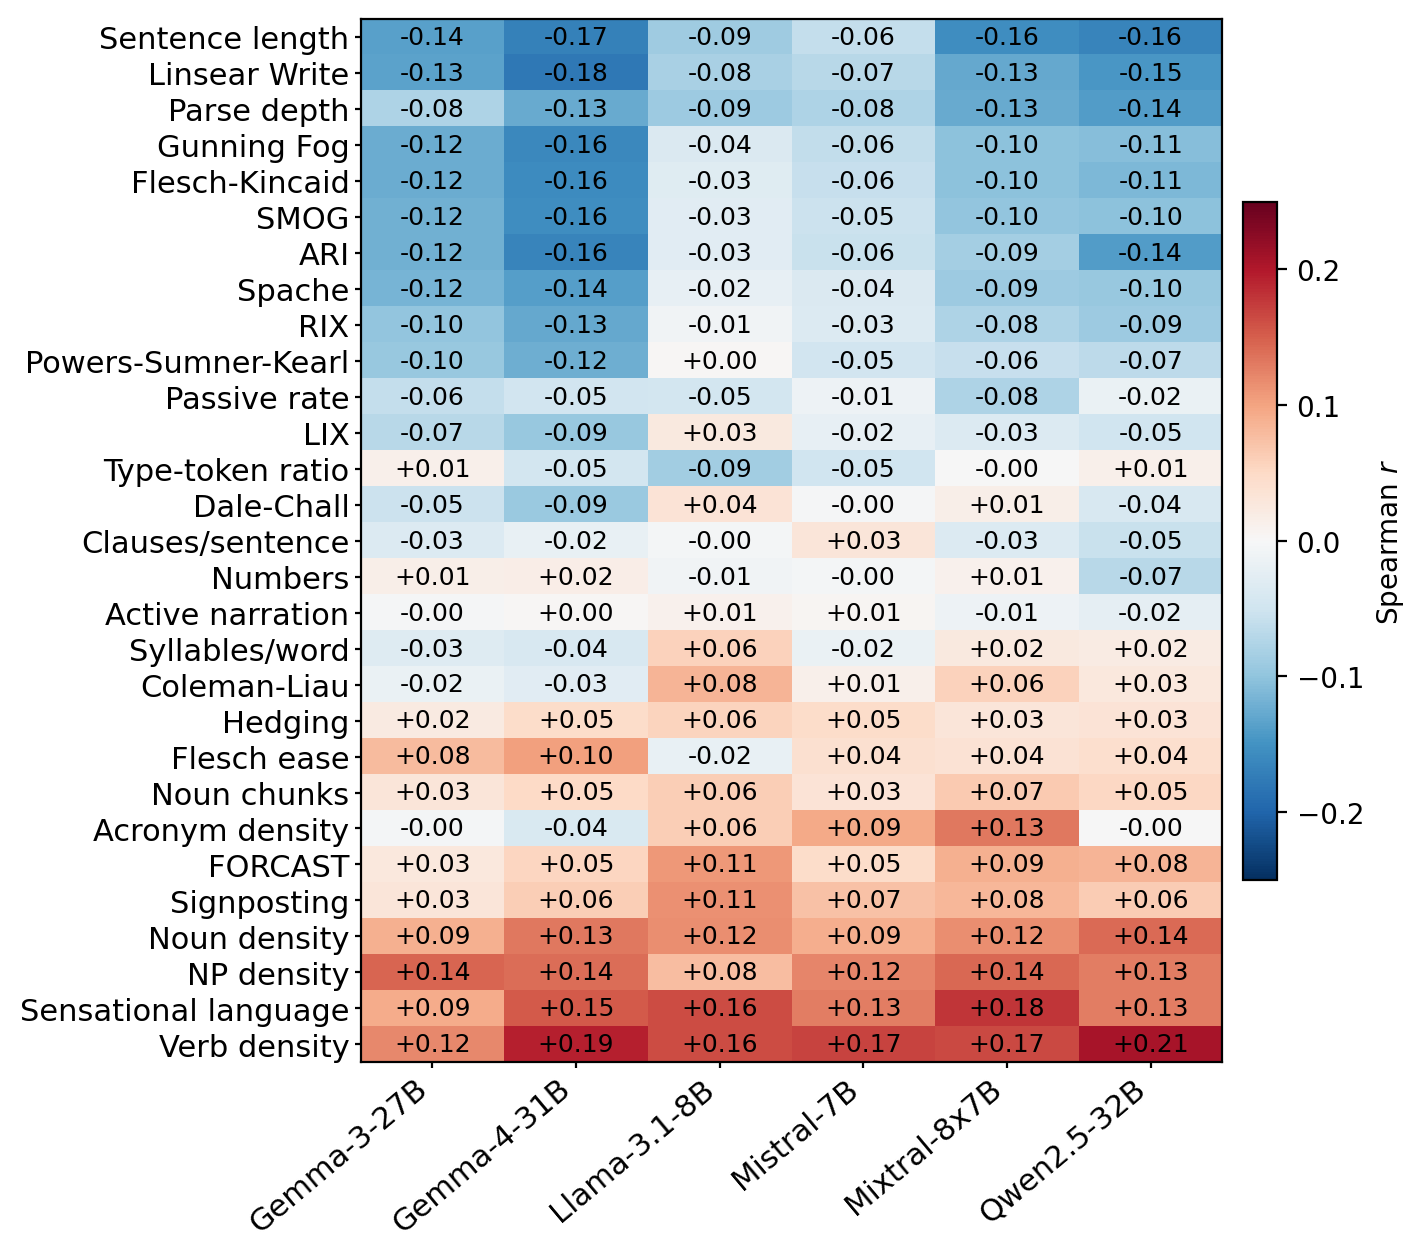
\includegraphics[width=0.72\textwidth]{figs/fig_judge_metric_heatmap.png}
\caption{\textbf{Per-paper correlation between writing metrics and judge
  score.} Spearman
  correlation between each writing metric and each model's judge score, over
  24,754 NeurIPS abstracts. A model's score for an abstract is the median of
  its nine generations, three prompts by three sampled runs. Rows are sorted
  by the correlation with the mean of those six per-model scores
  (1987--2024, the years the judge was scored). The judge score runs 1 to 5
  with higher meaning easier, so each cell's sign says which way that feature
  moves the judge. \textbf{Red (positive): more of that feature is judged
  \emph{more} readable}, as for verb density, sensational language and noun
  phrase density. \textbf{Blue (negative): more of it is judged \emph{less}
  readable}, as for sentence length and syntactic complexity, which is the
  direction the classical formulas also take. Near-white cells, including
  acronym density, indicate near indifference. All values are Spearman
  correlations and every effect is small ($|r| < 0.25$).}
\label{fig:judge-tracks}
\end{figure*}


\end{document}
